%!TEX program = xelatex

\documentclass[a4paper, openany, oneside]{memoir}
\usepackage[no-math]{fontspec}
\usepackage{pgfplots}
\pgfplotsset{compat=newest}
\usepackage{commath}
\usepackage{mathtools}
\usepackage{amssymb}
\usepackage{amsthm}
\usepackage{booktabs}
\usepackage{mathtools}
\usepackage{xcolor}
\usepackage[separate-uncertainty=true, per-mode=symbol]{siunitx}
\usepackage[noabbrev, capitalize]{cleveref}
\usepackage{listings}
\usepackage[american inductor, european resistor]{circuitikz}
\usepackage{amsmath}
\usepackage{amsfonts}
\usepackage{ifxetex}
\usepackage[dutch,english]{babel}
\usepackage[backend=bibtexu,texencoding=utf8,bibencoding=utf8,style=ieee,sortlocale=en_GB,language=auto]{biblatex}
\usepackage[strict,autostyle]{csquotes}
\usepackage{parskip}
\usepackage{import}
\usepackage{standalone}
\usepackage{hyperref}
%\usepackage[toc,title,titletoc]{appendix}

\ifxetex{} % Fonts laden in het geval dat je met Xetex compiled
    \usepackage{fontspec}
    \defaultfontfeatures{Ligatures=TeX} % To support LaTeX quoting style
    \setromanfont{Palatino Linotype} % Tover ergens in Font mapje in root.
    \setmonofont{Source Code Pro}
\else % Terug val in standaard pdflatex tool chain. Geen ondersteuning voor OTT fonts
    \usepackage[T1]{fontenc}
    \usepackage[utf8]{inputenc}
\fi
\newcommand{\references}[1]{\begin{flushright}{#1}\end{flushright}}
\renewcommand{\vec}[1]{\boldsymbol{\mathbf{#1}}}
\newcommand{\uvec}[1]{\boldsymbol{\hat{\vec{#1}}}}
\newcommand{\mat}[1]{\boldsymbol{\mathbf{#1}}}
\newcommand{\fasor}[1]{\boldsymbol{\tilde{\vec{#1}}}}
\newcommand{\cmplx}[0]{\mathrm{j}}
\renewcommand{\Re}[0]{\operatorname{Re}}
\newcommand{\Cov}{\operatorname{Cov}}
\newcommand{\Var}{\operatorname{Var}}
\newcommand{\proj}{\operatorname{proj}}
\newcommand{\Perp}{\operatorname{perp}}
\newcommand{\col}{\operatorname{col}}
\newcommand{\rect}{\operatorname{rect}}
\newcommand{\sinc}{\operatorname{sinc}}
\newcommand{\IT}{\operatorname{IT}}
\newcommand{\F}{\mathcal{F}}

\newtheorem{definition}{Definition}
\newtheorem{theorem}{Theorem}


\DeclareSIUnit{\voltampere}{VA} %apparent power
\DeclareSIUnit{\pii}{\ensuremath{\pi}}

\hypersetup{%setup hyperlinks
    colorlinks,
    citecolor=black,
    filecolor=black,
    linkcolor=black,
    urlcolor=black
}

% Example boxes
\usepackage{fancybox}
\usepackage{framed}
\usepackage{adjustbox}
\newenvironment{simpages}%
{\AtBeginEnvironment{itemize}{\parskip=0pt\parsep=0pt\partopsep=0pt}
\def\FrameCommand{\fboxsep=.5\FrameSep\shadowbox}\MakeFramed{\FrameRestore}}%
{\endMakeFramed}

% Impulse train
\DeclareFontFamily{U}{wncy}{}
\DeclareFontShape{U}{wncy}{m}{n}{<->wncyr10}{}
\DeclareSymbolFont{mcy}{U}{wncy}{m}{n}
\DeclareMathSymbol{\Sha}{\mathord}{mcy}{"58}
\addbibresource{../../../../includes/bibliography.bib}

\begin{document}

\section{Optimisation}
In this section we will look at each sampling method and examine ways to optimise each of them.

\todo[inline, author=Kees]{hier moet een stuk dat wessels stuk linkt aan het oplossen van simpele wiskunde problemen}

\section{Circular sparse ruler}
We introduce the concept of a ruler. Consider a ruler $\vec{r}$ of length $N$. Then $\vec{r} \in \{0,1\}^N$. Also, $(\vec{r})_i = 1$ if the element at position $i$ is marked, and $(\vec{r})_i = 0$ if the elements at position is not marked. We will formulate the minimal circular ruler problem as an binary integer linear program.

A ruler $\vec{r}$ contains a distance $d$ if there exist $i$ and $j$ such that $(\vec{r})_i = 1$, $(\vec{r})_j = 1$ and $|i-j| = d$ or  $N-|i-j| = d$. The ruler $\vec{r}$ is a circular ruler if it contains distances $ 1, \ldots, N - 1$. A circular ruler $\vec{r}$ is minimal if and only if $||\vec{r}||_1$ is minimal. A circular ruler can be depicted in a nice way. \Cref{fig:circular-ruler} shows a minimal circular ruler for $N=7$. The circle depicts the ruler and contains $N$ ticks. Then $(\vec{r})_i = 1$ if the tick at position $i$ is red. The definition of a circular ruler then states that the ruler is circular if and only if the distances between the marks are the distances $1,\ldots,N-1$.

In circular sparse ruler we have different samplers with the same sampling frequency $N$. Therefore the sampling structure is periodic with  period $N$.
If we can make lag $L$ we can also make lag $L+kN$ with $k \in \mathbb{Z}$. Therefore if we can make lags $\{0,1,\dots,N-1\}$, we can make all lags in $\mathbb{Z}$. Because of this we only need to look at how to acquire the lags $\{0,1,\dots,N-1\}$. This problem is called circular sparse ruler. We construct a circle with $N$ marks on it. Every mark can be occupied by a sampler. Time on this circle passes as the hand of a clock. the distance between two samplers on the circle is equal to the lag one would get. This is illustrated in \cref{fig:circular-ruler}, where $N=7$, and the samplers occupy the locations $\{1,2,4\}$.

\begin{figure}[H]
    \centering
    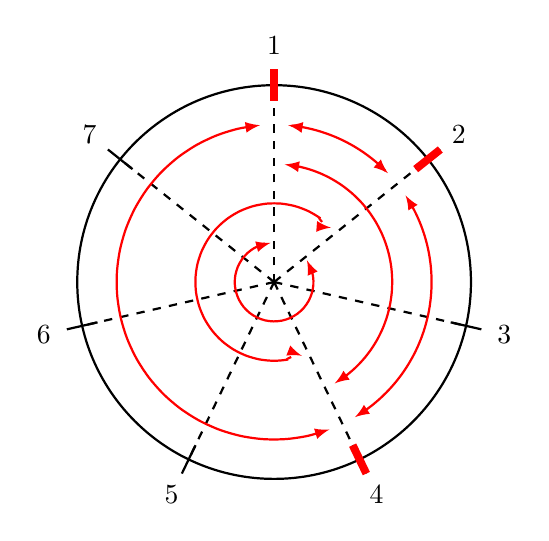
\begin{tikzpicture}
        \def\N{7}
        \draw [thick, black] circle[radius=2.5cm] (0,0);
        \foreach \i in {1,...,\N} {
            \draw [scale=1,domain=2.3:2.7,smooth,variable=\x,black,thick] plot ({\x*sin(360*(\i-1)/\N)},{\x*cos(360*(\i-1)/\N)});
            \draw [black,thick,dashed] (0,0) -- ({2.5*sin(360*(\i-1)/\N)},{2.5*cos(360*(\i-1)/\N)});
            \node[black] at ({3*sin(360*(\i-1)/\N)},{3*cos(360*(\i-1)/\N)}) {$\i$};
        }
        \foreach \i in {0,1,3} {
            \draw [scale=1,domain=2.3:2.7,smooth,variable=\x,red,line width=1mm] plot ({\x*sin(360*\i/\N)},{\x*cos(360*\i/\N)});
        }
        \draw [scale=1,domain=0.1:0.9,smooth,variable=\x,black,thick,>=latex,<->,red] plot ({2*sin(360*\x/\N)},{2*cos(360*\x/\N)}); % 1
        \draw [scale=1,domain=1.1:2.9,smooth,variable=\x,black,thick,>=latex,<->,red] plot ({2*sin(360*\x/\N)},{2*cos(360*\x/\N)}); % 2
        \draw [scale=1,domain=3.1:6.9,smooth,variable=\x,black,thick,>=latex,<->,red] plot ({2*sin(360*\x/\N)},{2*cos(360*\x/\N)}); % 4
        \draw [scale=1,domain=0.1:2.9,smooth,variable=\x,black,thick,>=latex,<->,red] plot ({1.5*sin(360*\x/\N)},{1.5*cos(360*\x/\N)}); % 3
        \draw [scale=1,domain=3.1:7.9,smooth,variable=\x,black,thick,>=latex,<->,red] plot ({1*sin(360*\x/\N)},{1*cos(360*\x/\N)}); % 5
        \draw [scale=1,domain=1.1:6.9,smooth,variable=\x,black,thick,>=latex,<->,red] plot ({0.5*sin(360*\x/\N)},{0.5*cos(360*\x/\N)}); % 6
    \end{tikzpicture}
    \caption{Minimal circular ruler for $N=7$}
    \label{fig:circular-ruler}
\end{figure}

The larger down-sampling factor $N$ with the same $M$ amount of samplers, the better the performance. Finding good solutions for this problem is therefore a convenient optimization for our device. D.Ariananda and G.Leus \todo{ref}, proposed a solution that uses linear sparse ruler to generate solution for the circular sparse ruler problem. The linear sparse ruler problem is identical to the circular sparse ruler, but the only one period is considered. Therefore the ends do not connect, as is illustrated in \cref{tkz:linear_sparse_ruler}.  

\begin{figure}[H]
\centering
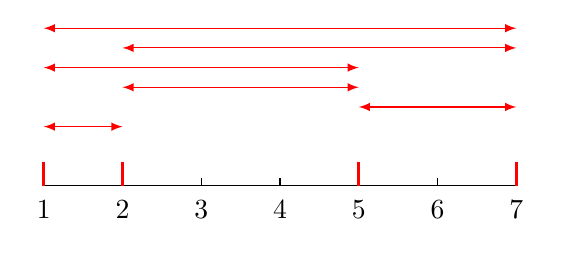
\begin{tikzpicture}

\draw (0,1) -- (6,1);

\draw [red, very thick] (0,1) -- (0,1.3);
\draw [red, very thick](1,1) -- (1,1.3);
\draw (2,1) -- (2,1.1);
\draw (3,1) -- (3,1.1);
\draw [red, very thick](4,1) -- (4,1.3);
\draw (5,1) -- (5,1.1);
\draw [red, very thick](6,1) -- (6,1.3);

\draw [red, >=latex,<->] (0,1.75) -- (1,1.75);
\draw [red, >=latex,<->](4,2) -- (6,2);
\draw [red, >=latex,<->](1,2.25) -- (4,2.25);
\draw [red, >=latex,<->](0,2.5) -- (4,2.5);
\draw [red, >=latex,<->](1,2.75) -- (6,2.75);
\draw [red, >=latex,<->](0,3) -- (6,3);

\node at (0,0.7) {1};
\node at (1,0.7) {2};
\node at (2,0.7) {3};
\node at (3,0.7) {4};
\node at (4,0.7) {5};
\node at (5,0.7) {6};
\node at (6,0.7) {7};

\end{tikzpicture}
\caption{linear sparse ruler with $N=7$ and $M=4$}\label{tkz:linear_sparse_ruler}
\end{figure}

The proposed method in ref \todo{ref}   is that a linear sparse solution for $N=x$ is also a circular sparse ruler solution for $N=2(x-1)$ when $x$ is even, and $N=2x-1$ when $x$ is odd. This can be readily seen, because for every lag $L_i<\lfloor\frac{N}{2}\rfloor$, there is also a lag $L_j = N-L_i$. The linear sparse solution in \cref{tkz:linear_sparse_ruler} of $\{1,2,5,7\}$ with $N=7$, is therefore also a circular sparse ruler solution for $N=13$ as is illustrated in \cref{tkz:linear_sparse_ruler}. 

\begin{figure}[H]
\centering
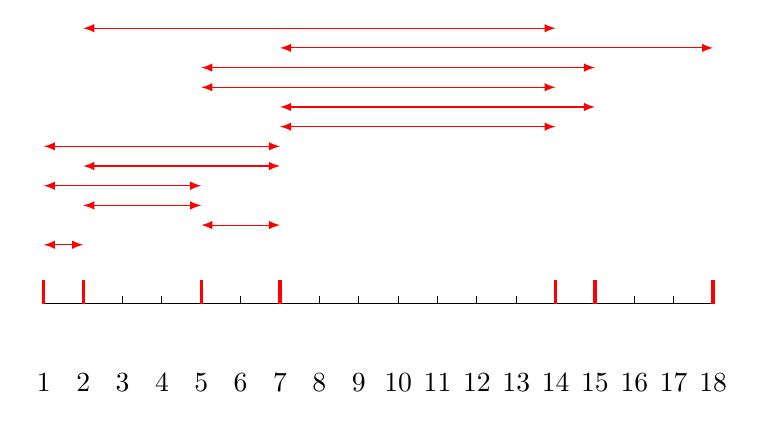
\begin{tikzpicture}

\draw (0,1) -- (8.5,1);

\draw [red, very thick] (0,1) -- (0,1.3);
\draw [red, very thick](.5,1) -- (.5,1.3);
\draw (1,1) -- (1,1.1);
\draw (1.5,1) -- (1.5,1.1);
\draw [red, very thick](2,1) -- (2,1.3);
\draw (2.5,1) -- (2.5,1.1);
\draw [red, very thick](3,1) -- (3,1.3);
\draw  (3.5,1) -- (3.5,1.1);
\draw (4,1) -- (4,1.1);
\draw (4.5,1) -- (4.5,1.1);
\draw (5,1) -- (5,1.1);
\draw (5.5,1) -- (5.5,1.1);
\draw (6,1) -- (6,1.1);

\draw [red, very thick] (6.5,1) -- (6.5,1.3);
\draw [red, very thick](7,1) -- (7,1.3);
\draw (7.5,1) -- (7.5,1.1);
\draw (8,1) -- (8,1.1);
\draw [red, very thick](8.5,1) -- (8.5,1.3);

\draw [red, >=latex,<->] (0,1.75) -- (.5,1.75);
\draw [red, >=latex,<->](2,2) -- (3,2);
\draw [red, >=latex,<->](.5,2.25) -- (2,2.25);
\draw [red, >=latex,<->](0,2.5) -- (2,2.5);
\draw [red, >=latex,<->](.5,2.75) -- (3,2.75);
\draw [red, >=latex,<->](0,3) -- (3,3);
\draw [red, >=latex,<->](3,3.25) -- (6.5,3.25);
\draw [red, >=latex,<->](3,3.5) -- (7,3.5);
\draw [red, >=latex,<->](2,3.75) -- (6.5,3.75);
\draw [red, >=latex,<->](2,4) -- (7,4);
\draw [red, >=latex,<->](3,4.25) -- (8.5,4.25);
\draw [red, >=latex,<->](.5,4.5) -- (6.5,4.5);

\node at (0,0) {1};
\node at (.5,0) {2};
\node at (1,0) {3};
\node at (1.5,0) {4};
\node at (2,0) {5};
\node at (2.5,0) {6};
\node at (3,0) {7};
\node at (3.5,0) {8};
\node at (4,0) {9};
\node at (4.5,0) {10};
\node at (5,0) {11};
\node at (5.5,0) {12};
\node at (6,0) {13};
\node at (6.5,0) {14};
\node at (7,0) {15};
\node at (7.5,0) {16};
\node at (8,0) {17};
\node at (8.5,0) {18};

\end{tikzpicture}
\caption{circular sparse solution for $N=13$}\label{tkz:circ_linear_sparse}
\end{figure}

This approach has one main advantage: solutions for linear sparse ruler can be recycled into circular sparse ruler solutions, and better linear sparse ruler solutions will also result in better circular sparse ruler solutions. Because linear sparse ruler is a well known problem, good solutions are easy to come by. However, the solutions generated are not necessarily optimal. There might be situations in which one can do better than with linear sparse ruler solutions. This problem is by no means trivial and requires clever algorithms to calculate. It is also interesting to look at the structure of the problem to decrease the solution space.

\subsection{Structure of circular sparse ruler}
We are looking for optimal circular sparse rulers. Optimal circular sparse rulers are circular sparse ruler solutions with $M$ sampler and a down-sampling factor of $N$, if and only if there exist no solution with the same $M$ samplers, but higher $N$. Optimal solutions ensure the highest performance possible for given amount of samplers. In similar fashion can one define optimal linear sparse ruler. 

\begin{blockTheorem}[Upper bound circular sparse ruler]\label{th:upperbound}
the down-sampling factor $N$ of a circular sparse ruler solution with $M$ devices cannot be more than $N=M(M-1)+1$. 
\end{blockTheorem}

To see why \cref{th:upperbound} holds, we take a look at the maximum amount of different combinations of $$m_i-m_j, \quad m_i, m_j \in M,$$ which is $M^2$. We know that for $M$ combinations we have $m_i=m_j$, resulting in lag 0. This means that we have at least $M-1$ double lags. $$M^2-M+1 = M(M-1)+1$$

For example: observe that an optimal linear sparse ruler for $M=5$, is $\{1,2,5,8,10\}$ with $N=10$, resulting in a circular sparse ruler solution with $N=19$. However the circular sparse ruler solution $\{1,2,7,9,19\}$ with $N=21$ is better, and also optimal, because the upper bound for $M=5$ is $N=21$ as dictated in \cref{th:upperbound}. This example illustrates the potential for increased performance in circular sparse ruler. 

One circular sparse ruler can be used to make $2N-1$ other circular sparse ruler solutions through translation and mirroring the solution. The first $N-1$ solutions can be made by translating all positions over the circle with $N$ positions. The other $N$ solutions can be made by first mirroring the solution on the circle, and then translating the new solution in similar fashion over the circle. To lose some redundancy we consider these variations to be identical.    

\subsection{Integer linear programming (ILP)}
\begin{blockTheorem} \label{th:ruler-distance}\nolinebreak
    Let $\vec{r} \in \{0,1\}^N$ be a ruler. Then $\vec{r}$ contains the distance $d$ if $\vec{d}^T \vec{r} = 2$ for any $\vec{d} \in D_d$.\nolinebreak
\end{blockTheorem}

\begin{blockProofTheorem}{\ref{th:ruler-distance}}
    Assume that $\vec{d}^T\vec{r} = 2$. Then there exist $i$ and $j$ such that $(\vec{d})_i (\vec{r})_i + (\vec{d})_j (\vec{r})_j = 2$. This implies that $(\vec{r})_i = 1$ and $(\vec{r})_j = 1$. Since $\vec{d} \in D_d$, either $|i-j|=d$ or $|i-j| = N-d$. In both cases, $\vec{r}$ contains the distance $d$. 
\end{blockProofTheorem}

Let $\mat{D}_d$ denote the $|D_d| \times N$ matrix which contains all vectors in $D_d$ as rows.

\begin{blockTheorem} \label{th:ruler-distance-matrix}\nolinebreak
    Let $\vec{r} \in \{0,1\}^N$ be a ruler and let $\vec{y} \in \{0,1\}^{|D_d|}$. Then $\vec{r}$ contains the distance $d$ at least once if $\mat{D}_d \vec{r} \ge 2\vec{y}$ such that $||\vec{y}||_1 = 1$.
\end{blockTheorem}

\begin{blockProofTheorem}{\ref{th:ruler-distance-matrix}}
    Assume that $\mat{D}_d \vec{r} \ge 2 \vec{y}$ such that $||\vec{y}||_1 = 1$. Then there is one and only one $i$ such that $(\vec{y})_i=1$. Therefore there exists a $\vec{d} \in D_d$ such that $\vec{d}^T \vec{r} \ge 2 (\vec{y})_i = 2$. Since $||\vec{d}||_1=2$, the equality holds and thus $\vec{r}$ contains the distance $d$. Now consider $\vec{d}' \in D_d$ such that $\vec{d}' \neq \vec{d}$. Then $\vec{d}^T \vec{r} \ge 0$, which holds for any $\vec{r}$.  
\end{blockProofTheorem}

Consider the binary integer linear program
\begin{align*}
    \text{minimise } &\vec{1}_N^T \vec{r} \\
    \text{such that } &
    \begin{bmatrix}
        \mat{D}_1 \\
        \vdots \\
        \mat{D}_{N-1}
    \end{bmatrix} \vec{r} \ge 2 \begin{bmatrix}
        \vec{y}_1 \\
        \vdots \\
        \vec{y}_2
    \end{bmatrix}, \begin{bmatrix}
        \vec{1}_{|D_1|}^T & & \\
        & \ddots & \\
        & & \vec{1}_{|D_{N-1}|}^T
    \end{bmatrix}  \begin{bmatrix}
        \vec{y}_1 \\
        \vdots \\
        \vec{y}_{N-1}
    \end{bmatrix} = \vec{1}_{N-1}, \\
    & \vec{r} \in \{0,1\}^N \text{ and } \vec{y}_i \in \{0,1\}^{|D_i|} \text{ for } i = 1,\ldots,N-1.
\end{align*}
Then, by the definition of a minimal circular ruler and \cref{th:ruler-distance-matrix}, this program yields a minimal circular ruler of length $N$.

\subsection{results}
Using this program we generated a set of circular sparse ruler solutions.
\begin{align}
M=2,N=3  \quad S&=\{1,2\}\\
M=3,N=7  \quad S&=\{1,2,4\}\\
M=4,N=13 \quad S&=\{1,2,5,7\}\\
M=5,N=21 \quad S&=\{1,2,7,9, 19\}\\
M=6,N=31 \quad S&=\{1,2,5,7,14,22\}\\
M=7,N=39 \quad S&=\{1,2,5,7,14,21,31\}\\
M=8,N=51 \quad S&=\{1,2,8,9,12,21,31\}\\
M=9,N=61 \quad S&=\{1,2,5,7,11,23,31, 38, 49\}
\end{align}

to be continued...


\end{document}
